\chapter{RISC-V}
\label{ch6_riscv}

\section{Introduction}
 \label{sect6_1}
 
The performance derived from a computer and the amount of energy that is consumed in the process hugely depends on algorithms, application code, compiler, microarchitecture, Instruction Set Architecture (ISA), physical design, circuit design and fabrication process. This is the order of abstraction from a user working on the computer, starting from the top most layer exposed to programmer, down to the bottom most layer which depends on how the chip is fabricated. \newline\newline
The Central Processing Unit (CPU) is one of the most significant parts of any computing device, as it is the brain of the computer \cite{riscv_xda}. It performs arithmetic and logical operations and moves data from one place to another. This is done by the processor according to ISA it is based on. An ISA is a well-defined interface linking computer software to the hardware its running on, enabling the independent development of the two computing realms. It is strictly an interface specification, not an implementation. \newline\newline
In today's age, technology has been able to evolve much more because of the existence of open standards and open source software – Linux as an open source operating system for example. This builds the case for an ISA which is not proprietary and is powerful enough to drive custom processing chips. \newline\newline
Historically, ISAs have been proprietary for business reasons, but there is no good technical reason for the absence or deficiency of open source ISAs. Having a free and open source ISA specification would hugely benefit the industry, just like how open source software has added great value. It would directly lead to a rise in innovation via free-market competition, with several designers coming with various implementations, which comprise both the open source and proprietary ISA versions. More shared open core designs would exist, reducing the time taken to hit the market, lowering cost from reuse, and making the designs more transparent and error-free. Moreover, an open ISA would lead to processors becoming affordable for a greater number of devices, helping in expanding the Internet of Things (IoTs) \cite{riscv_isa_free}.

\subsection{About}
 \label{sect6_1_1}
RISC-V is an ISA originally designed to support computer architecture research and education, now reaching the stage to become a standard open architecture for industry implementations, under the governance of the RISC-V foundation. It was developed in the Computer Science Division of the EECS department at University of California, Berkeley \cite{riscv_home}. Its development was inspired by ARM's IP restrictions together with the lack of 64-bit addresses. \newline\newline
RISC-V has learned from various mistakes in different ISAs, making its design superior to other ISAs incorporating a better mix of capabilities \cite{riscv_isa_free}. It provides a small core instruction set that compilers and operating systems can depend on, as well as optional standard extensions. It has a compact instruction set encoding – smaller code is desirable as it reduces the memory requirement. It offers single, double and quadruple precision floating point capabilities, in addition to being 32, 64 and 128-bit addressable. \newline\newline
RISC-V was defined with a goal to be completely open and freely open to academic researchers and industries. Designed with small, fast and low-power real-word implementations in mind, it does not over-architect for a particular style of microarchitecture. It is a real ISA suited for direct native hardware implementation, not for just simulation or binary translation. It provides support for the revised 2008 IEEE-754 floating-point standard \cite{ieee_754}. RISC-V simplifies experiments with new supervisor-level and hypervisor-level ISA designs. \newline\newline
RISC-V's capabilities make it extremely powerful, yet simple and clean to implement. In contrast to most ISAs, it is available for all types for use, empowering anyone to design, manufacture and sell RISC-V chips and software. It supports small embedded systems, Personal Computers (PCs), supercomputers with vector processors, and warehouse-scale rack mounted parallel computers. Thus, the widespread usage of RISC-V would allow software developers to target an open hardware target, while making commercial processor designers compete on implementation superiority. 

\subsection{ISA Specifications}
 \label{sect6_1_2}
RISC-V is specified as a base integer ISA, which is a must in any implementation, with additional extensions to the base ISA. Based on the width of the integer registers, the base instruction set has two variants, RV32I and RV64I. There is scope for a future variant RV128I for 128-bit address support \cite{riscv_isa_manual}. It provides support for extensive customization and specialization, along with extension beyond the base instruction set, but doesn't allow redefining these base integer instructions. \newline\newline
There are four core instruction formats defined in the base instruction set, as shown follows:
\begin{figure}[h!]
\centering
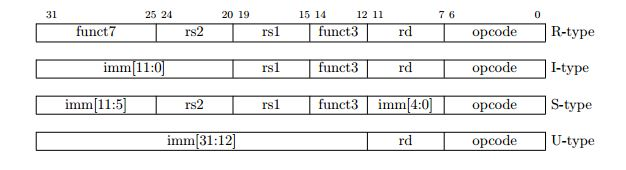
\includegraphics[width=\linewidth]{figures/RV32I_Instruction_Types.JPG}
\caption{Base instruction formats in RISC-V \cite{riscv_tools_bootcamp}}
\label{fig:riscv1}
\end{figure}

Furthermore, there are two variations of the instruction formats (SB/UJ) based on how immediate values are taken care of. A few sets of standard extensions have been pre-defined to cater to general software development. These comprise integer multiplication/division (extension “M”), atomic operations (extension “A”), single-precision floating-point (extension “F”), and double-precision floating-point (extension “D”). A combination of these 4 standard extensions (“IMAFD”) is given a general abbreviation of “G”, which results in a general-purpose scalar instruction set. RV32G and RV64G are currently set as default targets of the RISC-V compiler toolchains. The base set and extensions have been kept separated to have a simple instruction set. \newline\newline
The base integer instruction set for the 32-bit and 64-bit variants (RV32I/\\RV64I) comprises 40 instructions, while the general-purpose instruction set (RV32G/RV64G) supports 122 instructions. There are 31 general purpose registers x1-x31 capable of storing integer values, register x0 being hardwired to the constant value 0. The register width is 32 bits for RV32I and 64 bits for RV64I. RISC-V is based on the load-store architecture, where arithmetic operations only function on the data stored the registers and only the load and store operations access memory. The user address space is byte-addressed and little-endian. \newline\newline
There also exists a reduced version of the base integer instruction set (RV32I), designed specifically for embedded systems (denoted by “E”). The major difference is that the number of registers in RV32E is reduced to 16 from 31 in RV32I. A draft proposal for the RISC-V standard compressed instruction set has been made which reduces static and dynamic code size by adding short 16-bit instruction encodings for conventional operations. Denoted by the extension “C”, it could be added to any of the base ISA variants (RV32I, RV64I, and RV128I). 

 \section{Software Tools and Setup Required}
  \label{sect6_2}

\subsection{Software Tools}
 \label{sect6_2_1}
Several software tools and libraries are required to be downloaded and setup before any development on RISC-V can begin. A meta-repository is available on GitHub, with Git submodules containing every stable component of the RISC-V software toolchain \cite{riscv_tools_bootcamp}. The image below shows the software stack of riscv-tools: 
\begin{figure}[h!]
\centering
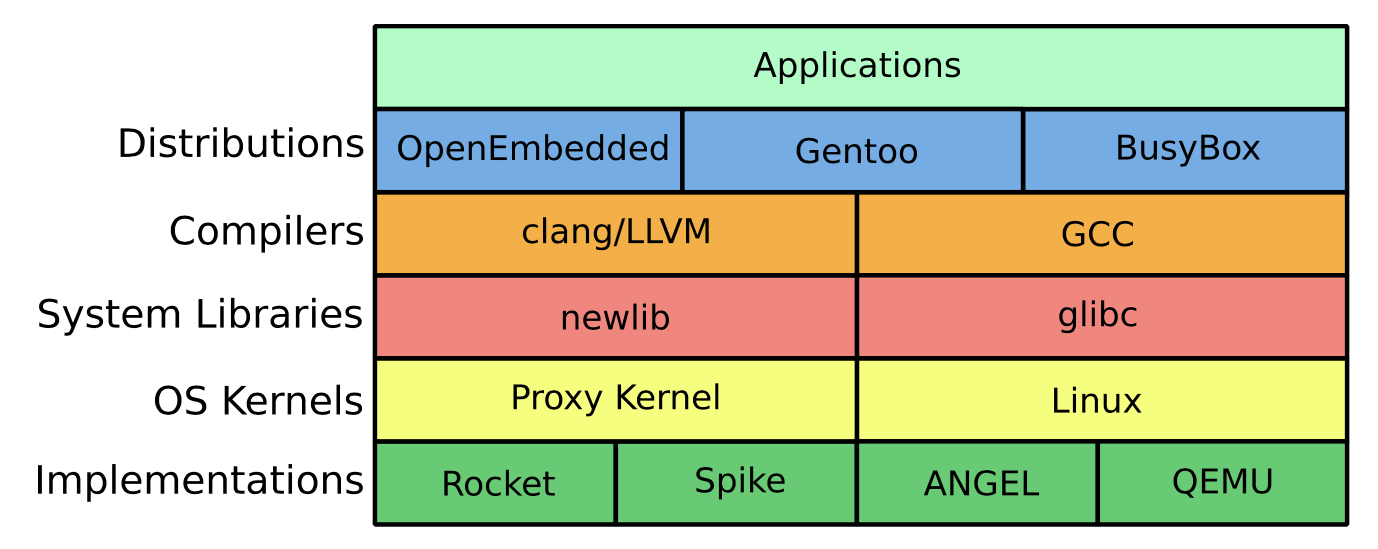
\includegraphics[width=\linewidth]{figures/RISC-V_Software_Stack.png}
\caption{Software stack for RISC-V tools \cite{riscv_tools_bootcamp}}
\label{fig:riscv2}
\end{figure}

\subsubsection{GNU Toolchain}
 \label{sect6_2_1_1}
The RISC-V GNU Toolchain is a RISC-V C and C++ cross compiler utility. It contents include binutils, gcc, newlib, glibc, and Linux UAPI headers. It supports two build modes: a generic ELD/Newlib toolchain and a more sophisticated Linux-ELF/glibc toolchain. The riscv-unknown-elf command is used to compile a program while riscv64-unknown-elf-gcc is used to assemble and link with gcc/binutils.

\subsubsection{Front End Server}
 \label{sect6_2_1_2}
RISC-V front end server library facilitates communication between the host machine and the RISC-V target device on the Host-Target Interface (HTIF). It also provides a virtualized console and disk device \cite{riscv_soft_tools}. 

\subsubsection{Proxy Kernel}
 \label{sect6_2_1_3}
RISC-V proxy kernel is responsible for servicing system calls generated by code built and linked with the RISC-V Newlib port \cite{riscv_soft_tools}. It handles system calls like open, close and printf. Abbreviated as \verb|pk| (or \verb|riscv-pk|), it is a lightweight application execution environment that can host statically-linked RISC-V ELF binaries. It is designed to support tethered RISC-V implementations with limited I/O capability and thus handles I/O-related system calls by proxying them to a host computer \cite{riscv_pk}.

\subsubsection{ISA Simulator}
 \label{sect6_2_1_4}
RISC-V ISA simulator consists of a functional simulator known as Spike \cite{riscv_soft_tools}. It implements a functional model of one or more RISC-V processors \cite{riscv_isa}. Since there is no proper operating system, it executes the generated binary running on top of the proxy kernel. \newline\newline
Spike takes the path of the binary to run as its argument, which is \verb|pk|, located at \verb|$RISCV/riscv-elf/bin/pk| and finds it automatically. The name of the program to be run is the argument for \verb|riscv-pk|, which then executes the program. An interactive debug mode can be invoked in Spike with the -d command line flag or \verb|SIGINT|, which enables single-stepping through instructions, setting break point conditions, printing register and memory contents, etc.

\subsubsection{Opcodes}
 \label{sect6_2_1_5}
RISC-V Opcodes is a subcomponent of riscv-tools which enumerates all standard RISC-V instruction opcodes executable by the simulator, and control and status registers (CSRs). It also has a script to convert them into different formats (C, Scala, LaTex) \cite{riscv_opcodes}.

\subsection{Setup Required}
 \label{sect6_2_2}
There are many possible combinations to pick for the different layers of the stack shown in Figure 4, but there exist 2 of the most common workflows for RISC-V software development \cite{riscv_tools_bootcamp}. These are as follows:
\begin{itemize}
\item \textbf{Spike + pk} \newline
The use case for following this workflow are embedded or single applications.
\begin{itemize}
\item Distributions: None
\item Compilers: clang/LLVM or GCC
\item System Libraries: newlib
\item OS Kernels: Proxy Kernel (pk)
\item Implementations: Spike
\end{itemize}	
	
\item \textbf{QEMU + Linux} \newline
The use case for following this workflow is Simple POSIX environment.
\begin{itemize}
\item Distributions: BusyBox
\item Compilers: GCC
\item System Libraries: glibc
\item OS Kernels: Linux
\item Implementations: QEMU
\end{itemize}
\end{itemize}
In this case, the former workflow was followed, the aim being familiarization with the RISC-V development phase. The selected workflow was easier to set up and took lesser time. This requires the components riscv-gnu-toolchain, riscv-fesvr, riscv-isa-sim, and riscv-pk. \newline\newline
The binaries generated against newlib system library will not be running on a full-blown operating system, but will require access to few crucial system calls \cite{riscv_soft_tools}. The setup will thus require the installation of riscv-newlib. Newlib is a C library intended for embedded systems. It has the edge of not being unnecessarily complicated over Glibc, as well as having sufficient support. Also, its porting process is much simpler than that of Glibc because it only requires a few stubs of glue code. These stubs of code include the system calls that are supposed to call into the operating system you're running on.

\subsubsection{Toolchain}
\label{sect6_2_2_1}
The following steps were followed to obtain and compile the RISC-V toolchain sources for the above-mentioned workflow:
\begin{enumerate}
\item To build GCC, several other Ubuntu packages like \verb|flex|, \verb|bison|, \verb|autotools|, \verb|libmpc|, \verb|libmpfr|, and \verb|libgmp| are required. Obtain the required Ubuntu packages required for installation with this command:\newline
\small \textbf{sudo apt-get install autoconf automake autotools-dev curl libmpc-dev libmpfr-dev libgmp-dev gawk build-essential bison flex texinfo gperf libtool patchutils bc}

\item Set the environment variables \verb|TOP| as the directory where the tools will be installed, i.e. the current working directory:\newline
\small \textbf{export \$TOP = \$(pwd)}

\item Clone riscv-tools repository from GitHub:\newline
\small \textbf{git clone https://github.com/riscv/riscv-tools.git}

\item Change into the \verb|riscv-tools| directory:\newline
\small \textbf{cd \$TOP/riscv-tools}

\item Instruct Git to update its submodules:\newline
\small \textbf{git submodule update –--init --recursive}

\item Set the \verb|RISCV| environment variable to point to the path where new tools will be installed:\newline
\small \textbf{export \$RISCV = \$TOP/riscv}

\item The \verb|PATH| environment variable also needs to be set to point to the directory specified by RISCV:\newline
\small \textbf{export \$PATH = \$PATH:\$RISCV/bin}

\item After everything has been set up, run the \verb|build| script:\newline
\small \textbf{./build.sh}
\end{enumerate}

A successful build marks the end of the toolchain installation process.

\subsubsection{Testing}
\label{sect6_2_2_2}
After the installation procedure is finished, testing was done to make sure that there were no issues with the set up. 
\begin{enumerate}
\item Change to the directory of toolchain installation:\newline
\small \textbf{cd \$TOP}
\item Write a simple “Hello World” program in a C file
%\small \textbf{echo \–e }\#include <stdio.h> '\n' int main(void) { printf(“Hello world!”); return 0; }’ \> hello.c
\item Build your program using the \verb|riscv64-unknown-elf-gcc| command:\newline
\small \textbf{riscv64-unknown-elf-gcc -o hello hello.c}
\item Run the binary on the ISA Simulator (Spike):\newline
\small \textbf{spike pk hello}
\end{enumerate}

The output generated should be "Hello world!", as shown below in Figure \ref{fig:riscv3} \newline

\begin{figure}[h!]
\centering
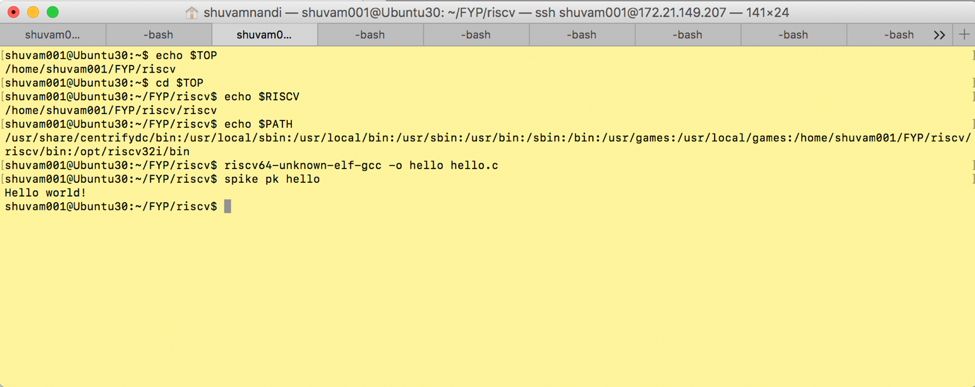
\includegraphics[width=\linewidth]{figures/Spike_Output.png}
\caption{Hello World program execution on Spike}
\label{fig:riscv3}
\end{figure}

 \section{PicoRV32}
  \label{sect6_3}
To understand how RISC-V is implemented in real, a processor implementation PicoRV32 was studied and analyzed. PicoRV32 is a processor core implementing the RV32IMC instruction set. It can be configured as RV32E, RV32I, RV32M, RV32C, or RV32IMC, and optionally contains a built-in interrupt controller. It is available free and is open sourced under the ISC license \cite{picorv32}. 

\subsection{About}
 \label{sect6_3_1}
PicoRV32 is a small sized processor which can operate at high frequencies (250-450 MHz on 7-Series Xilinx FPGAs). The core exists in two variants, \verb|picorv32| and \verb|picorv32_axi|. The former providing a simple native memory interface, easy to use in simple environments, while the latter providing an AXI-4 Lite Master interface that can be easily integrated with existing systems already using the AXI standard. It provides a selectable native memory interface, optional IRQ support and optional co-processor interface. This CPU core is designed to be added as an auxiliary processor in FPGA designs and ASICs. It could be easily integrated with most existing designs without exceeding clock domains. 

\subsection{Setup Required}
 \label{sect6_3_2}
PicoRV32 is based on the 32-bit version of RISC-V ISA, hence requires a setup of the complete toolchain targeting a pure RV32I CPU. 

\subsubsection{Toolchain}
 \label{sect6_3_2_1}
The following steps will download the toolchain required for programs to be compiled on PicoRV32 processor:

\begin{enumerate}
\item To build GCC, several other Ubuntu packages like \verb|flex|, \verb|bison|, \verb|autotools|, \verb|libmpc|, \verb|libmpfr|, and \verb|libgmp| are required. Obtain the required Ubuntu packages required for installation with this command:\newline
\small \textbf{sudo apt-get install autoconf automake autotools-dev curl libmpc-dev libmpfr-dev libgmp-dev gawk build-essential bison flex texinfo gperf libtool patchutils bc}

\item Create a new directory \verb|/opt/riscv32i| to store the toolchain once installed:
\newline
\small \textbf{sudo mkdir /opt/riscv32i}

\item Change permissions of the directory created in the previous step:\newline
\small \textbf{sudo chown \$USER /opt/riscv32i}

\item Obtain the toolchain from the riscv-tools GitHub repository of RISC-V foundation and store it in the directory \verb|riscv-gnu-toolchain-rv32i|:\newline
\small \textbf{git clone https://github.com/riscv/riscv-gnu-toolchain riscv-gnu-toolchain-rv32i}

\item Change into this directory:
\newline
\small \textbf{cd riscv-gnu-toolchain-rv32i}

\item Checkout the specific commit version:
\newline
\small \textbf{git checkout 914224e}

\item Update submodules within the repository:
\newline
\small \textbf{git submodule update --init --recursive}


\item Create a new directory \verb|build|:
\newline
\small \textbf{mkdir build}

\item Change into this directory:
\newline
\small \textbf{cd build}

\item Run the \verb|configure| script, which specifies the instruction set architecture as RV32I, and the directory to install the toolchain as /opt/riscv32i:
\newline
\small \textbf{../configure --with-arch=rv32i --prefix=/opt/riscv32i}

\item Run the \verb|make| script to build the toolchain:
\newline
\small \textbf{make -j\$(nproc)}
\end{enumerate}

\subsubsection{PicoRV32 Source Code}
 \label{sect6_3_2_2}
Now that the pure RV32I toolchain is downloaded, the CPU implementation can be downloaded and tested.

\begin{enumerate}
\item Clone PicoRV32 repository from GitHub:\newline
\small \textbf{git clone https://github.com/cliffordwolf/picorv32.git}

\item Run the \verb|make| script to build the toolchain:\newline
\small \textbf{cd \texttildelow /picorv32}

\item Run the \verb|make| script in the PicoRV32 source directory to download RV32IMC toolchains to be able to run all tests:\newline
\small \textbf{make -j\$(nproc) build-riscv32imc-tools - RV32IMC}

\end{enumerate}

\subsubsection{Icarus Verilog}
\label{sect6_3_2_3}
In order to test the working of the downloaded toolchain, the test bench provided by PicoRV32 must be run. This requires a software called \textit{Icarus Verilog}, which needs to be installed. Icarus Verilog is a Verilog simulation and synthesis tool. It operates as a compiler, compiling source code written in Verilog (IEEE-1364) into some target format. For batch simulation, the compiler can generate an intermediate form calledvvp assembly. This intermediate form is executed by the vvp command. For synthesis, the compiler generates netlists in the desired format \cite{iverilog_wil}. The following steps will download and install Icarus Verilog:

\begin{enumerate}
\item Clone the GitHub repository:\newline
\small \textbf{git clone https://github.com/steveicarus/iverilog.git}

\item Change into the \verb|iverilog| directory:\newline
\small \textbf{cd iverilog}

\item Update to the latest code in master branch:\newline
\small \textbf{git pull origin master}

\item Install \verb|autoconf| and \verb|gperf| packages installed for the configuration script to work (skip if step already done):\newline
\small \textbf{sudo apt-get install autoconf gperf}

\item Run \verb|autoconf.sh| script:\newline
\small \textbf{sh autoconf.sh}

\item Run \verb|configure| script:\newline
\small \textbf{./configure}

\item Run \verb|make| command with sudo access:\newline
\small \textbf{sudo make}

\item Run \verb|make| install:\newline
\small \textbf{make install}
\end{enumerate}

\subsection{Execution of Simple C Programs}
 \label{sect6_3_3}
After the installation of all tools required for using PicoRV32 was completed, the testbench provided was run by executing the make command. The following output was obtained:

\begin{figure}[h!]
\centering
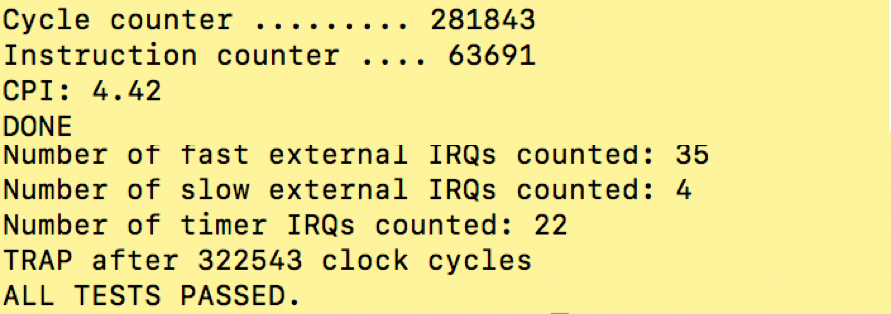
\includegraphics[width=\linewidth]{figures/PicoRV32_Execution.png}
\caption{Successful execution of PicRV32 testbench}
\label{fig:riscv4}
\end{figure}

This demonstrates that the installation was done successfully. The output is produced by different C files which are executed on the PicoRV32 CPU. The functions written in the C files are called in an assembly file \textit{start.S}, located in \verb|picorv32/firmware| directory. Along with C function calls, the assembly file also contains various tests in assembly files which get executed upon running make command. \newline
\begin{figure}[h!]
\centering
\includegraphics[height=15cm]{figures/PicoRV32_Compilation_Flow.png}
\caption{Compilation flow before execution on PicRV32}
\label{fig:riscv5}
\end{figure}

Upon further analysis of the compilation and execution flow, it was observed that the Icarus Verilog compiler compiles the \textit{testbench.v} and \textit{picorv32.v} files and generates an intermediate \verb|vvp| assembly file, \textit{testbench.vvp}. This is followed by the compilation of the \textit{start.S} assembly file, the C codes and test assembly files the into their binaries using the \verb|riscv32-unknown-el-| \\ \verb|f-gcc| command. This is succeeded by the generation of an executable file \textit{firmware.elf}, which is translated into a \textit{firmware.bin} file by \verb|riscv32-unknown-| \\ \verb|elf-objcopy| utility. In order to run the machine code on the processor, a script makehex.py in the firmware directory was used to convert the \textit{firmware.elf} file into \textit{firmware.hex} file. The \textit{firmware.hex} file contains instructions as defined by the RISC-V specification in the 32-bit format (represented as 8 digit hexadecimal numbers), which are passed to PicoRV32. The \verb|vvp| command of Icarus Verilog runs the previously generated \textit{testbench.vvp} file and executes the machine code on PicoRV32. The whole flow is shown as an activity diagram in Figure \ref{fig:riscv5}.\newline\newline
Observing the testbench output provided deep insights into how the execution maps from the high-level language C code to the low-level machine code. To understand how the processor executes these instructions, the Verilog file \textit{picorv32.v} was studied and understood. The instructions are loaded from the firmware.hex file in the testbench, which is stored in a 1024-bit wide register.
\begin{lstlisting}[language=Verilog]
reg [1023:0] firmware_file;
initial begin
end
if(!$value$plusargs("firmware=%s", firmware_file))
       firmware_file = "firmware/firmware.hex";
$readmemh(firmware_file, mem.memory);
\end{lstlisting}
The above code snippet shows the loading of the instructions into a 32-bit wide, 16384 lines long memory in an \verb|axi4_memory| instance. The instance is declared as follows:\newline
\begin{lstlisting}[language=Verilog]
reg [31:0]   memory [0:64*1024/4-1];
\end{lstlisting}
This memory is the source of instructions for the processor, which lacks a default instruction memory. As mentioned in 5.3.1, PicoRV32 is available in two variants. In this case, the \verb|axi4_memory| is interfaced to the \verb|picorv32_axi| version of PicoRV32 core, using the \verb|picorv32_axi_adapter|. \newline\newline
Along with being the instruction source, this \verb|axi4_memory| memory instance acts as the data memory as well. This implies that PicoRV32 follows a \textbf{von Neumann} architecture with a unified memory for storing data and instructions. The assembly file \textit{start.S} is used to allocate specific parts of the memory instance to be used as data memory. This brings complexity in the form of management of different sections of the same memory for instruction and data storage purposes.\newline\newline
On an average, PicoRV32 was observed to have a Cycles Per Instruction (CPI) value of 4.8. The execution of some specific instructions increased the CPI. 

 \section{Implementation of RISC-V Processor}
 \label{sect6_4}
After understanding the working of PicoRV32 from a high-level perspective, the next step is to design and implement a small processor based on the RISC-V 32-bit base integer instruction set. PicoRV32 has several features, like custom instructions for IRQ handling, a unified memory for data and instructions, which make the processor complicated and heavier.

\subsection{Objective}
\label{sect6_4_1}
The objective is to develop a smaller and more efficient processor and analyze whether it could perform better than PicoRV32. The initial implementation intends to be capable of performing only a small set of instructions and compare its performance with PicoRV32. A fully functional processor implementing RISC-V ISA meeting the desired requirements (as mentioned in Section 6.4.2) must be developed before it could be further extended.\newline\newline
ModelSim SE-64 10.5 was used for implementing the RISCVProcessor in Verilog.
\subsection{Design}
\label{sect6_4_2}
\subsubsection{Requirements}
\label{section:sect6_4_2_1}
The design of any RISC based processor follows the load-store architecture. This would be a 32-bit variant of the base integer instruction set, meaning that the registers width would be 32 bits. It would support instructions from the base integer instruction set and the multiplication extension (RV32IM). To start off with, the following instructions need to be present in our RISC-V implementation:
\begin{itemize}
\item Arithmetic: ADD, ADDI, MUL
\item Load/Store: LW, SW
\item Jump: JAL
\item Branch: BNE
\end{itemize}
Among the above instructions, ADD, MUL, fall into the category of R-type instructions; ADDI and LW fall into the I-type instruction category, SW is in the S-type instruction category; JAL is in the UJ-type instruction category; BNE uses the SB-type instruction format. \newline\newline
Harvard architecture is selected over von Neumann architecture, as data and instruction memory separation is preferred. Two separate memory systems can perform better than having a single, unified memory for both data and instructions. The various components required by the processor implementation would be the control unit, registers, Arithmetic and Logic Unit (ALU) and instruction memory.

\subsubsection{Components}
\label{sect6_4_2_2}
The processor would be built using the required components as stated above in \ref{section:sect6_4_2_1}. This section discusses the functional requirements desired in the components.

\begin{enumerate}
\item \textbf{Registers} \newline
Under the RISC-V specification, the base integer instruction set has a set of 32 registers, each 32-bit wide (x1-x31, x0 hardwired to constant 0). The Control Unit decodes instructions and extracts the register address on which the ALU needs to perform specified instructions. Data can be transferred between memory and registers using the load and store instructions. Thus, in a load store architecture, register memory is significant and should be wisely used in order to reduce overheads of memory accesses. It can be declared as shown in the following code snippet:

\begin{lstlisting}[language=Verilog]
reg [31:0] regdata [0:31;
regdata[0] = 32'h0;  //Constant 0 stored in location 0
\end{lstlisting}

\item \textbf{Decode Unit} \newline
The decoder determines the meaning of each instruction the processor needs to perform. It fetches the instructions from the instruction memory, and extracts necessary information commanding the CPU what instruction must be performed on what data. \newline\newline
The decoder extracts the information of register addresses from which data needs to be accessed, as well as the operation required to be done. This is specified by the 7-bit \verb|opcode|, 3-bit \verb|func3| and 7-bit \verb|func7| bits in the 32-bit instruction, as seen in Figure \ref{fig:riscv1}.\newline\newline
The design of the decode unit needs to be done according to RISC-V instruction specifications, as seen in Figure \ref{fig:riscv6}. The \verb|func7| and \verb|func3| bits  distinguish several instructions. The \verb|opcode| can be same for various instructions, typically for the same class of instruction (R-type, I-type, etc.).

\begin{figure}[h!]
\centering
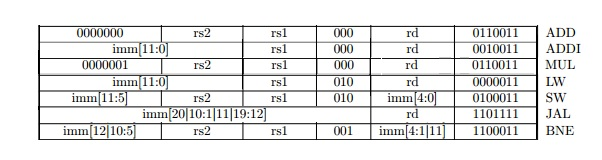
\includegraphics[width=\linewidth]{figures/RISCV_Instruction_Formats.jpg}
\caption{Formats for RISC-V instructions to be implemented \cite{riscv_isa_manual}}
\label{fig:riscv6}
\end{figure}

\item \textbf{Control Unit} \newline
The Control Unit determines the execution of operations on the processor. It instructs the processor's components like memory, ALU and input and output devices to respond to the program instructions. It can be perceived as the brain inside the CPU, making it the brain inside the brain of the computer. It is responsible for controlling the flow of data in specific ways for different instructions. This is done by signaling various flags which activate or deactivate different components of the CPU. \newline\newline
It consists of two registers, namely the Program Counter (PC) register and the Instruction Register (IR). PC points to the address of the instruction to be executed, while IR contains the instruction being currently interpreted. Instructions are fetched from the instruction memory and decoded in the Control Unit. The data required for the instruction to execute is extracted from the registers or data memory, and passed on to the ALU to perform the operation specified by the instruction opcode.

\item \textbf{Memory} \newline
Memory stores instructions and data. Being a Harvard Architecture processor, there would be a clear separation of instructions and data. A little endian memory system would be followed. The instruction memory stores the instructions generated by the makehex.py script, converting the firmware.bin file to firmware.hex format. The width and length of the instruction memory are 32 bits and 16384 lines, respectively. 

\item \textbf{Arithmetic and Logic Unit} \newline
The Arithmetic and Logic Unit of a CPU performs arithmetic and logical operations on operands specified by the instructions. It is the fundamental unit of the CPU of any computing device. After performing an operation, the result is stored back into the register file at the address specified by the instruction.

\begin{figure}[h!]
\centering
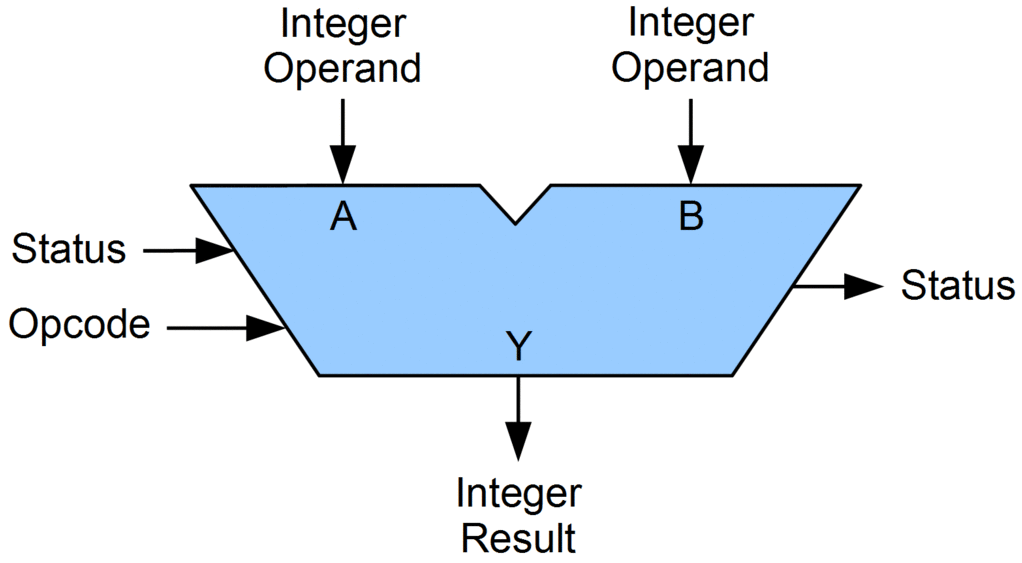
\includegraphics[width=8.5cm]{figures/ALU_block.PNG}
\caption{Symbolic representation of an ALU}
\label{fig:riscv7}
\end{figure}
\end{enumerate}

\subsection{Implementation Details}
\label{sect6_4_3}

\subsubsection{Testbench Simulation}
\label{sect6_4_3_2}

\subsubsection*{ADD}
\label{sect6_4_3_2a}

32-bit Instruction: 0x004100b3 \newline
Meaning: ADD R1, R2, R4 \newline

\begin{figure}[h!]
\centering
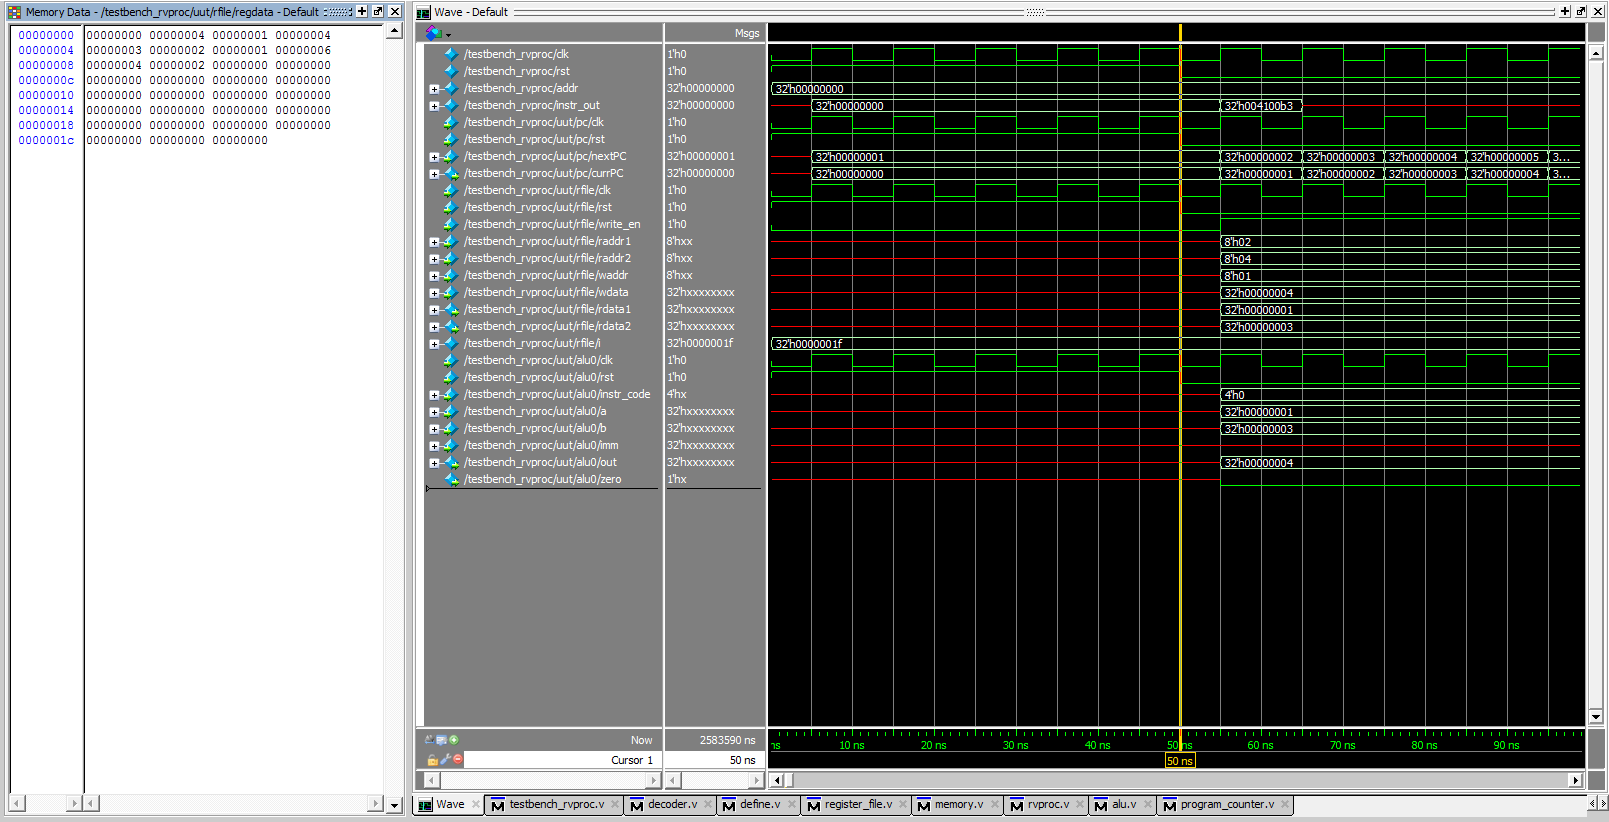
\includegraphics[width=\linewidth]{figures/RISCV_Implementation_ADD.PNG}
\caption{Testbench simulation result for ADD}
\label{fig:riscv9}
\end{figure}

\subsubsection*{MUL}
\label{sect6_4_3_2b}

32-bit Instruction: 0x024100b3 \newline
Meaning: MUL R1, R2, R4

\begin{figure}[h!]
\centering
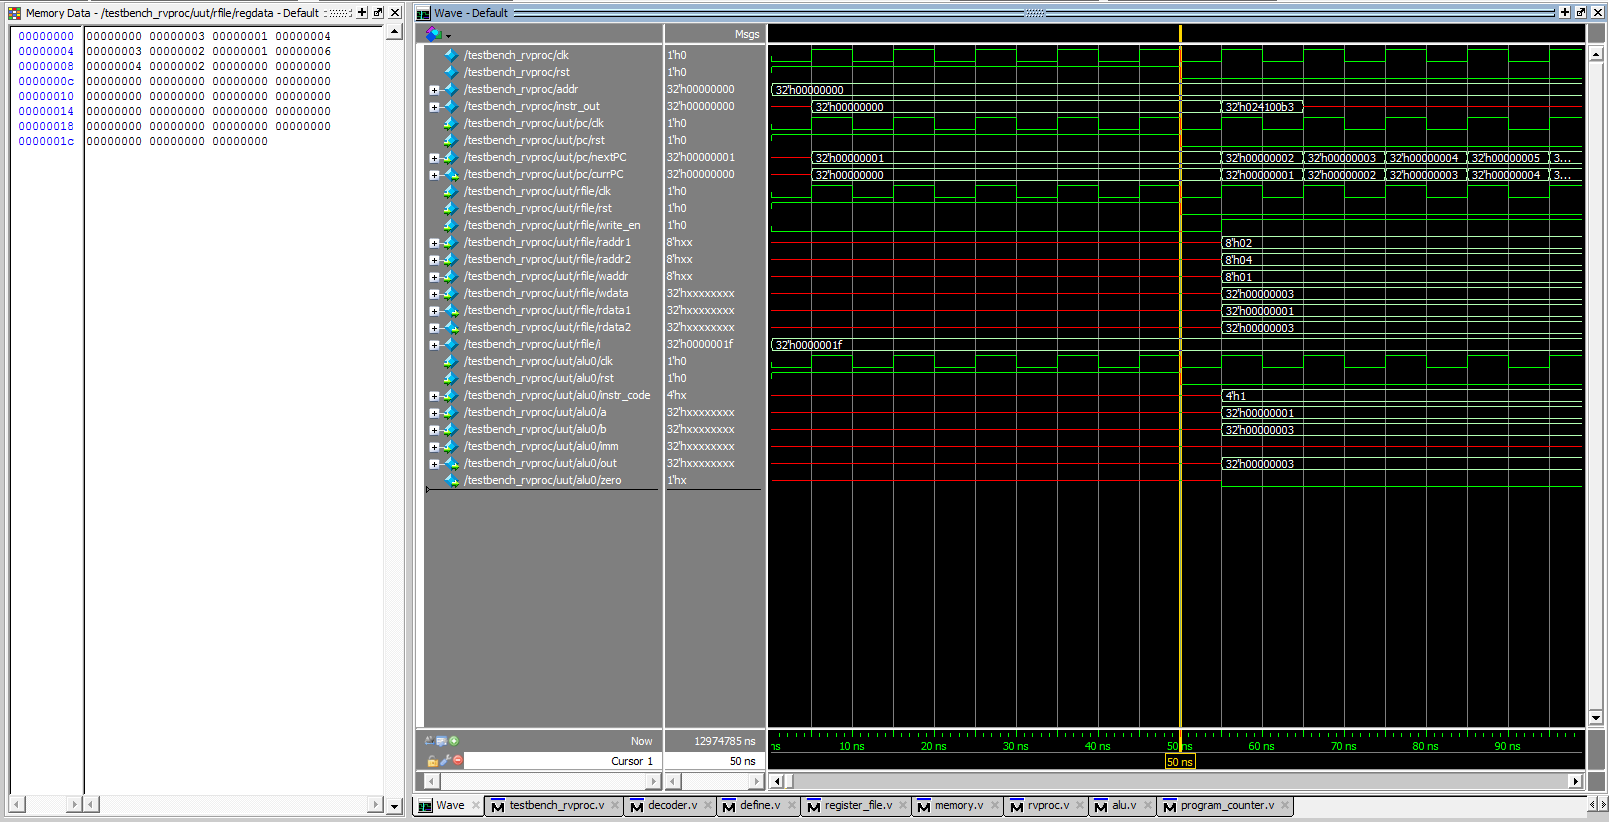
\includegraphics[width=\linewidth]{figures/RISCV_Implementation_MUL.PNG}
\caption{Testbench simulation result for MUL}
\label{fig:riscv10}
\end{figure}

\subsubsection*{ADDI}
\label{sect6_4_3_2c}

32-bit Instruction: 0x06418393 \newline
Meaning: ADDI R7, R3, \#100

\begin{figure}[h!]
\centering
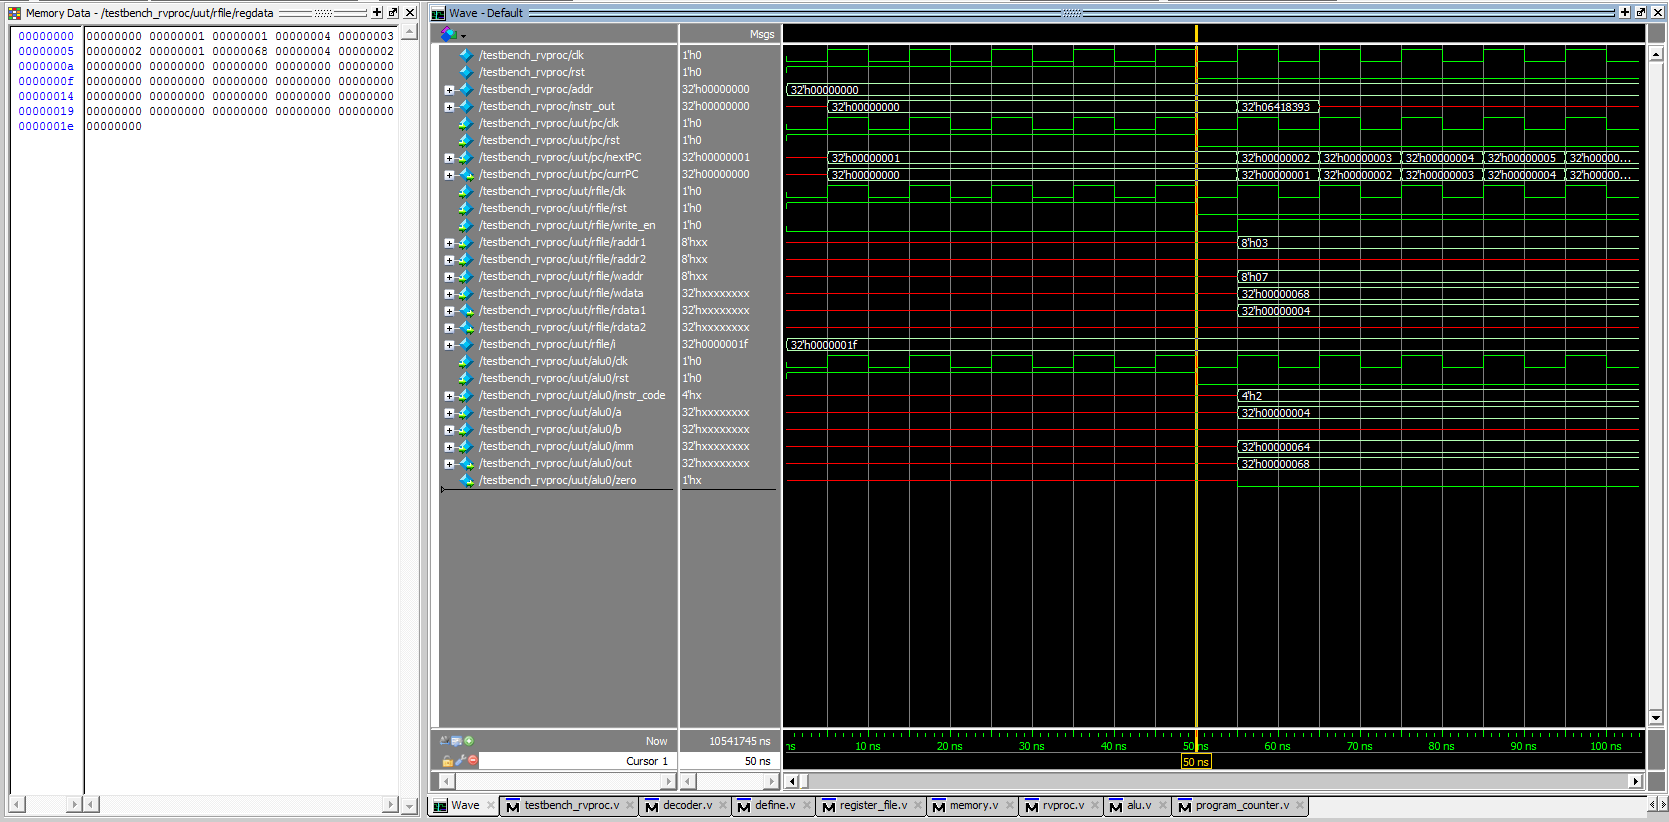
\includegraphics[width=\linewidth]{figures/RISCV_Implementation_ADDI.PNG}
\caption{Testbench simulation result for ADDI}
\label{fig:riscv11}
\end{figure}

\subsubsection*{LW}
\label{sect6_4_3_2d}

32-bit Instruction: 0x0000a283 \newline
Meaning: LW R5, [R1, \#0]

\begin{figure}[h!]
\centering
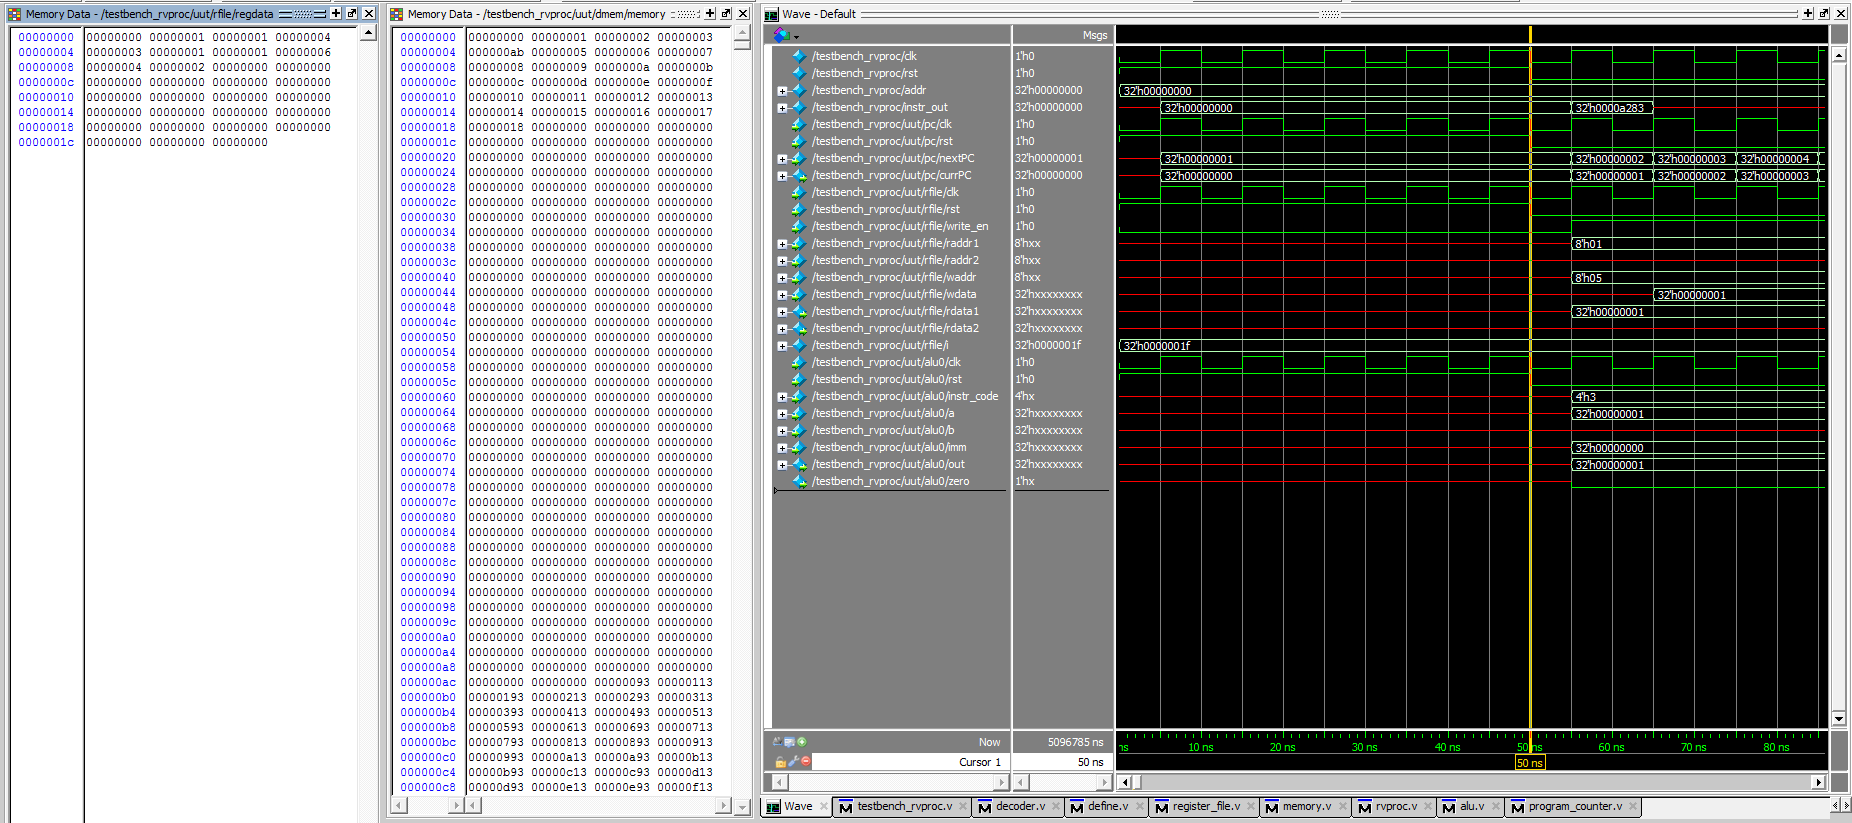
\includegraphics[width=\linewidth]{figures/RISCV_Implementation_LW.PNG}
\caption{Testbench simulation result for LW}
\label{fig:riscv12}
\end{figure}

\subsubsection*{SW}
\label{sect6_4_3_2e}

32-bit Instruction: 0x00522423 \newline
Meaning: SW R5, [R4, \#8]

\begin{figure}[h!]
\centering
%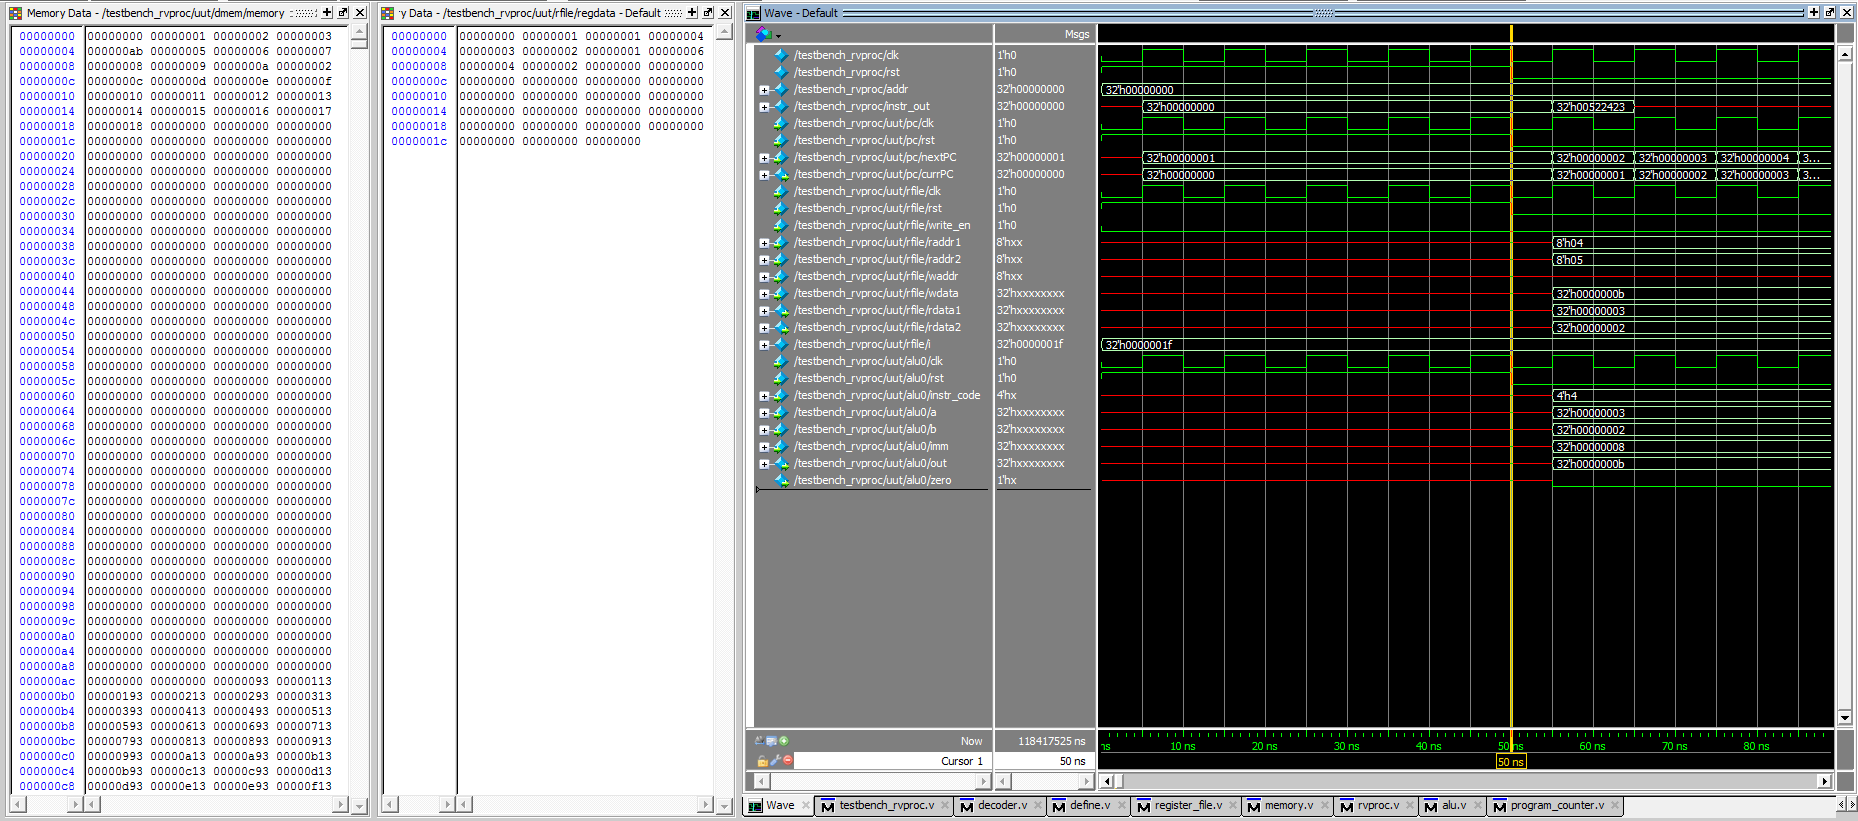
\includegraphics[width=\linewidth]{figures/RISCV_Implementation_SW.PNG}
\caption{Testbench simulation result for SW}
\label{fig:riscv13}
\end{figure}

\subsubsection*{BNE}
\label{sect6_4_3_2f}





